
HTBAC is a workflow system that uses RCT to implement ESMACS, and similar
protocols such as TIES\@. These protocols consist of pipelines with stages
comprised of heterogeneous tasks. For example, equilibration and production,
followed by post processing steps. The different protocols supported by HTBAC
differ in the details of the pipelines, stages and
synchronization~\cite{Bhati2017}.

\mtnote{I am not able to understand this paragraph so I am not able to propose
an alternative. I believe it should be rewritten.}\jhanote{OK?}

RADICAL-Cybertools provides advanced resource management capabilities and,
thereby delivers the necessary high- throughput capabilities required.HTBAC is
integrated with the EnTK component of RCT. EnTK provides a common API,
execution and programming model, thus allowing HTBAC to express the workflows
associated with different protocols uniformly, and thus minimize development
effort and complexity.

The Ensemble Toolkit API exposes four components (\textbf{Resource Handle},
\textbf{Pipeline}, \textbf{Stage}, and \textbf{Task}) to express the
application logic of HTBAC\@. We describe these components for the ESMACS
protocol\@. The concept of an ensemble in the ESMACS protocol maps directly to 
a set of pipelines in EnTK, where each pipeline contains functions that operate 
on a given replica. EnTK interprets these replicas as independent pipelines. 
Each pipeline consists of multiple stages representing a well-defined execution 
order; each stage can contain heterogeneous workloads. Although each stage of a 
pipeline depends on its predecessor, the pipelines execute independently of each 
other. The pattern within pipelines are identical and describes an ensemble of replica
simulations as shown in Fig~\ref{figure:ESMACS-pipelines}.

\jhanote{DWW, should we not use replica?}
\dwwnote{Shantenu, I have tried to make a consistent mapping above 
         and in the figure caption. Does this work for you?}\jhanote{cool!}

\begin{figure}
\centering
  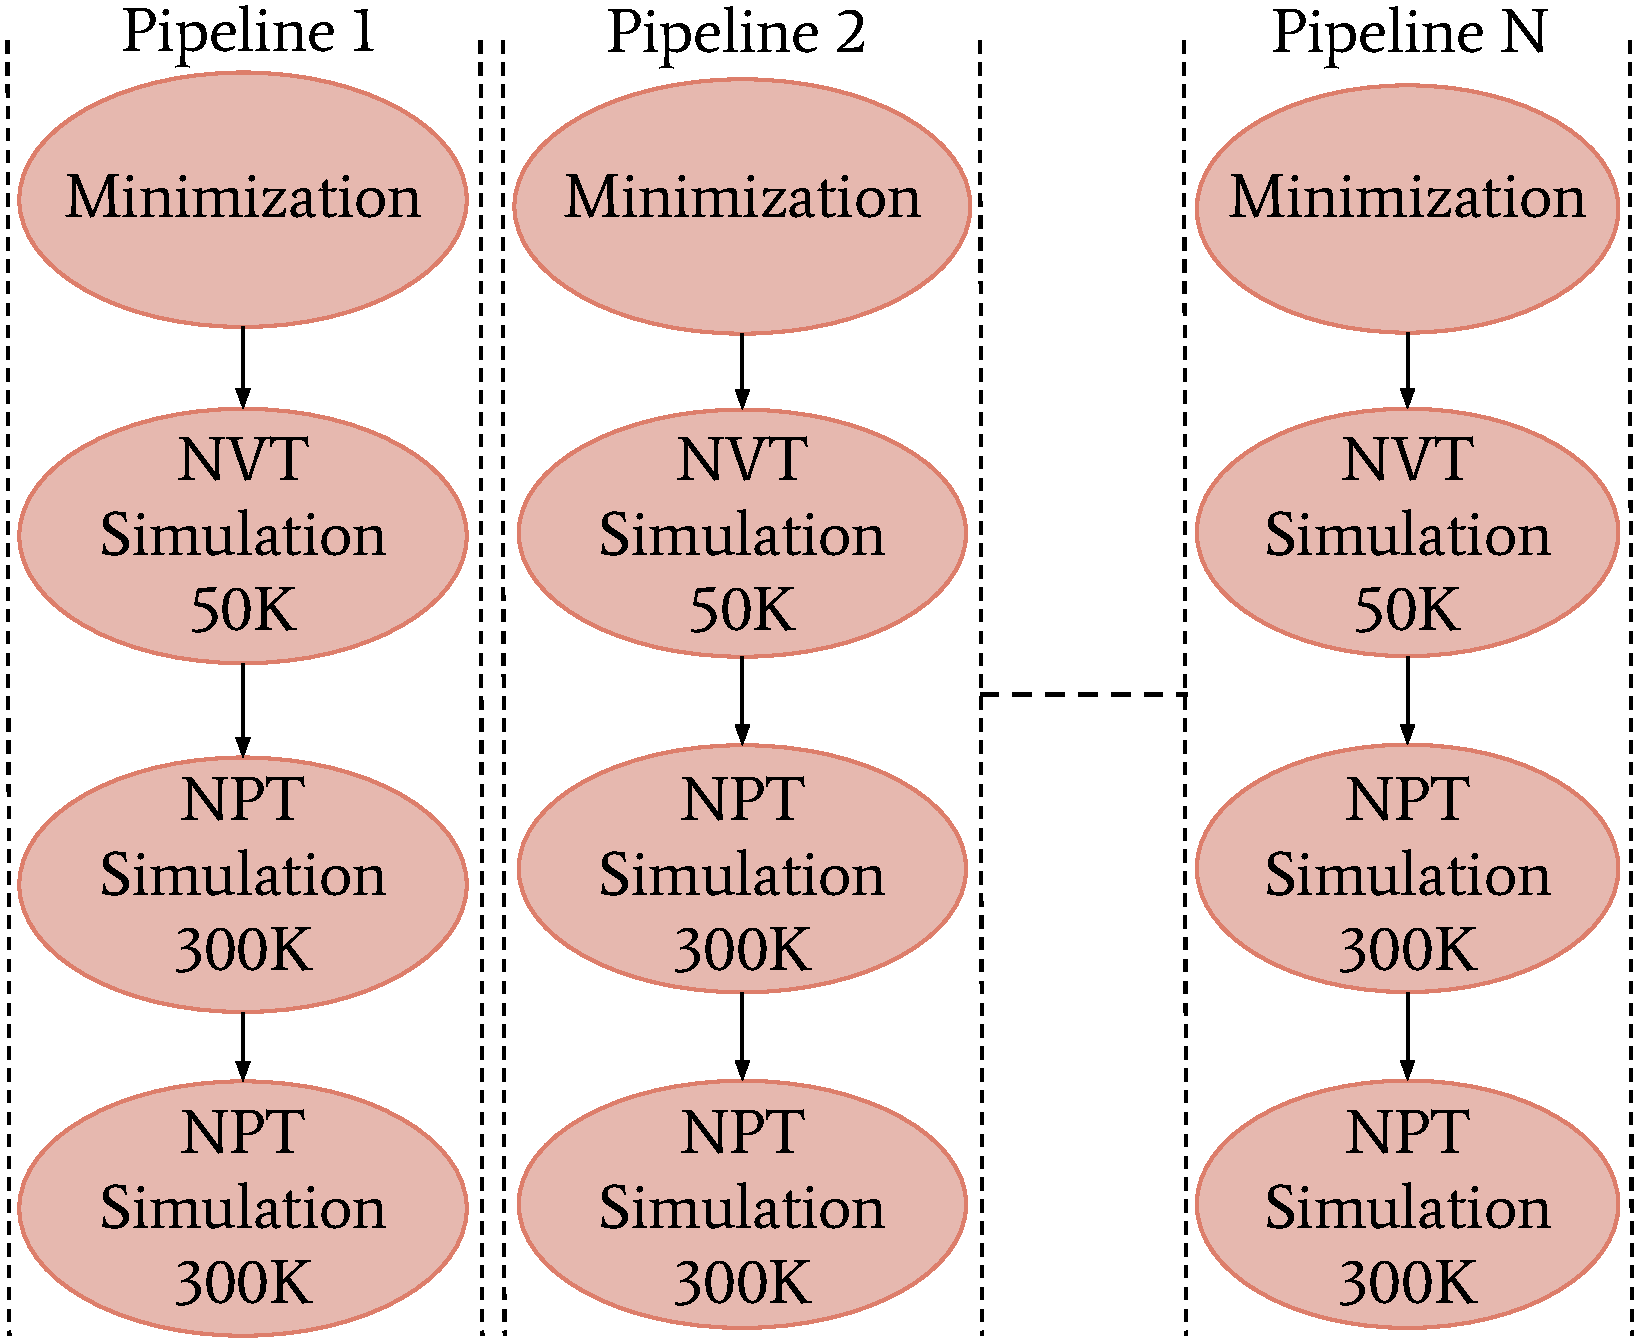
\includegraphics[width=0.5\textwidth]{FIGURES/HT-BAC_NAMD_pipelines_control_flow_only.pdf}
  \caption{ESMACS protocol indicating how an N replica ensemble is implemented in HTBAC.
  Each replica is mapped to a single EnTK pipeline. 
  Each pipeline is equivalent and represents a set of simulations which are captured as stages by
  EnTK.}\label{figure:ESMACS-pipelines}
\end{figure}

%\begin{itemize}
%	\item 1) Untar configuration files
%	\item 2) Preprep
%	\item 3) Minimize with decreasing restraints
%	\item 4) Equilibration: NVT simulation at 50K, with restraints
%	\item 5) Equilibration: NPT simulation at 300K, with decreasing
%	restraints
%	\item 6) Equlibratin: NPT at 300k, no constraints
%	\item 7) Tarball output files 
%\end{itemize}

Each stage is composed of a single unique task which is described by a set of
attributes that define the workload parameters such as the location of input
files, the number of simulations and the MD engine(s) to launch simulations.
The ESMACS protocol defines 7 stages, in which the preliminary and last
stages perform staging the input/output data. The middle stages indicate
simulation tasks as shown in Fig~\ref{figure:ESMACS-pipelines}. The task is
appended to a stage and stages are appended to a pipeline to maintain
temporal order. The workflow relies on a resource configuration which
consists of the details required to use a resource where the application will
be executed including runtime, queue, and account details. We capture the
integration of the application (ESMACS protocol) and how it interfaces with
EnTK in Fig~\ref{figure:ht-bac_rp}.

We define the client resource in Fig~\ref{figure:ht-bac_rp} as the workload
system---HTBAC which describes a series of replicas with ordered functions as
a pipelines with stages and tasks. EnTK interprets these pipelines as a
functional set of tasks and generates the pilot description that contains the
resource configuration of how to run the HTBAC workload. For the ESMACS
protocol running on Blue Waters we define the runtime system, queue, and the
pilot size. Once RADICAL-Pilot receives this new workload it generates a
pilot that submits placeholders to the queue. Once the pilot is activated,
the RP-Agent submits the tasks in the form of compute units to the
placeholders to begin execution.

\begin{figure}
\centering
  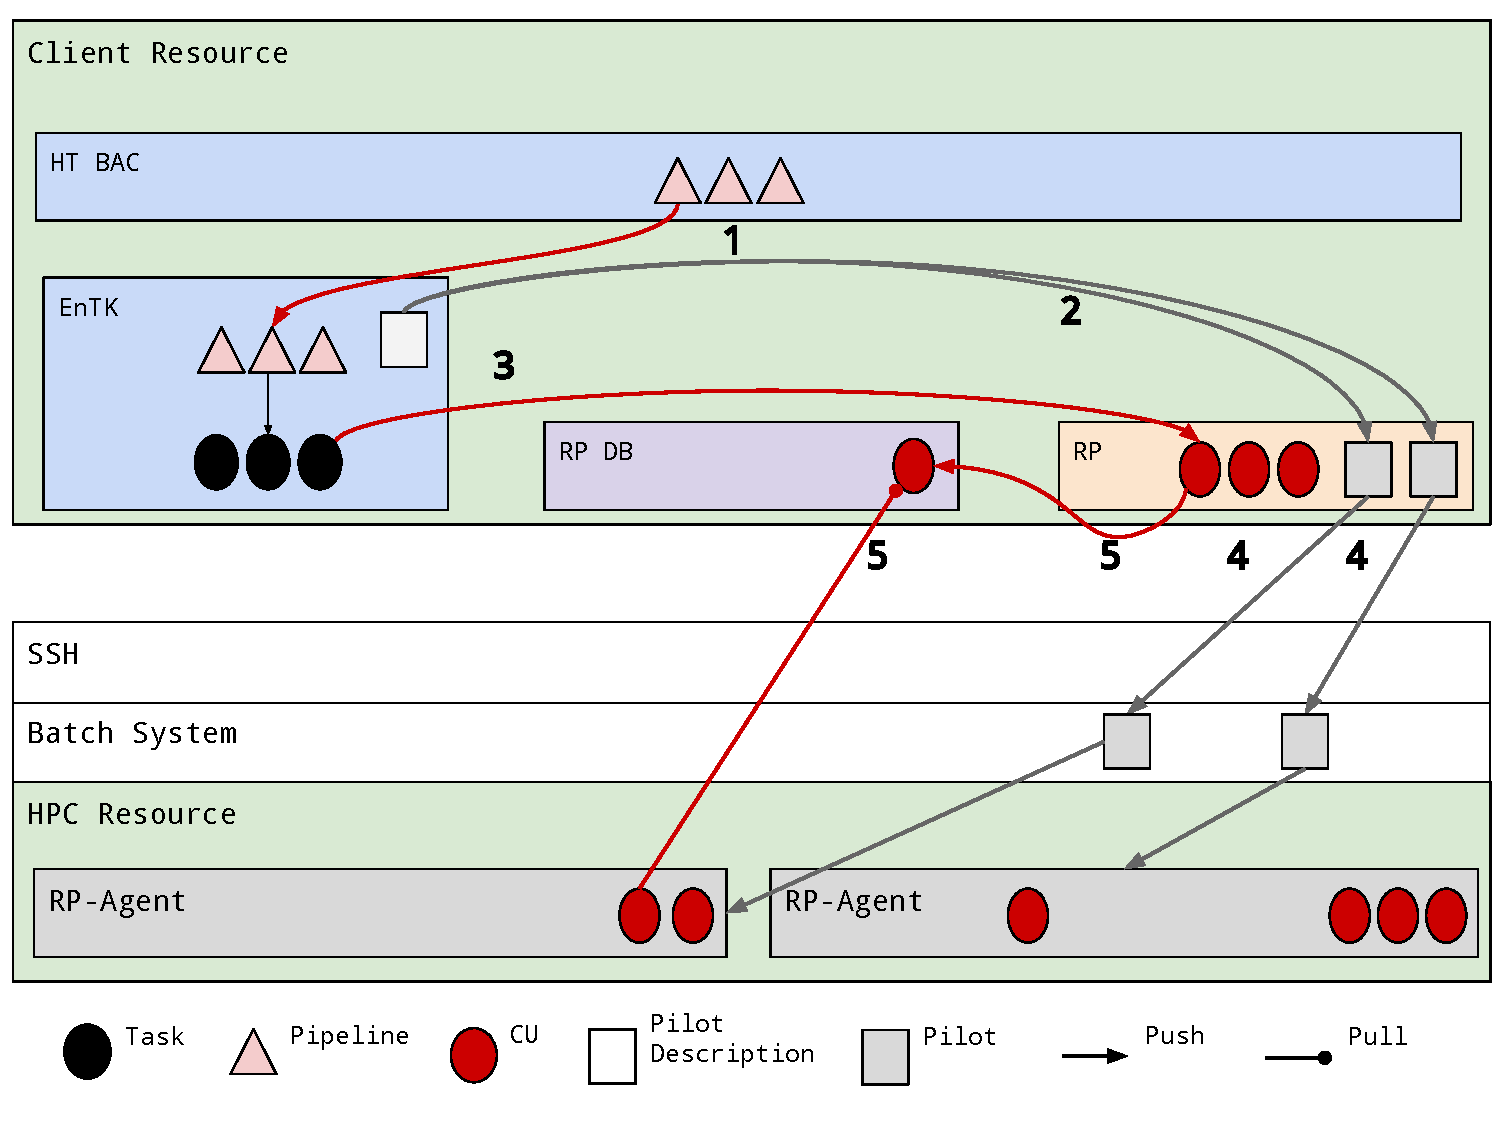
\includegraphics[width=0.5\textwidth]{FIGURES/ht-bac-rp_integration.pdf}
  \caption{\bf Integration between HTBAC workflow and EnTK\@. Numbers
  indicate the temporal sequence of execution. RADICAL-Pilot (RP) database
  (DB) can be deployed on any host reachable from the
  resources.\dwwnote{I think CU needs to be defined here}}\label{figure:ht-bac_rp}
\end{figure}



%\begin{figure}[ht]
%\centering
%  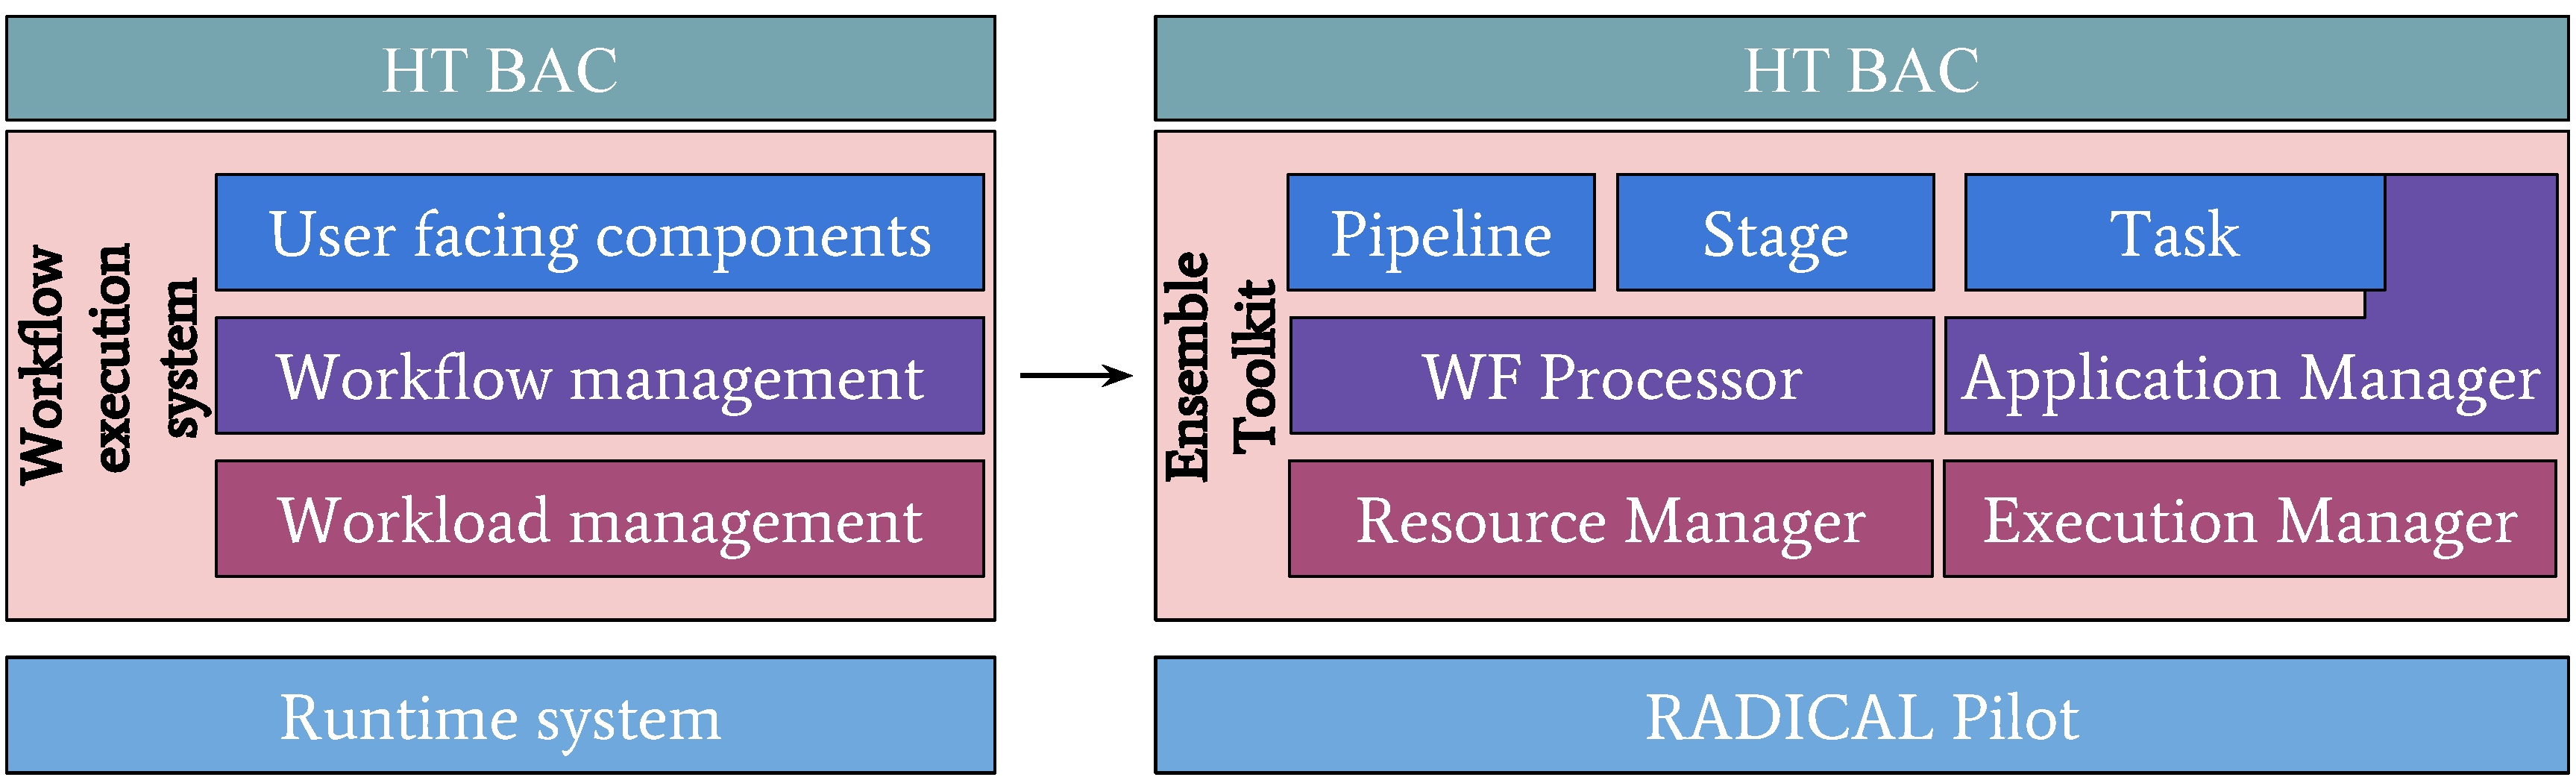
\includegraphics[width=0.5\textwidth]{FIGURES/entk_htbac_integration.pdf}
 % \caption{\bf Integration between HT-BAC workflow system and EnTK that shows resource/application managers.}
   %\label{figure:ht-bac_entk}
%\end{figure}

